\documentclass[12pt]{article}

% Essential packages for encoding, math, and formatting
\usepackage[utf8]{inputenc}
\usepackage[T1]{fontenc}
\usepackage{amsmath, amssymb, amsthm, mathtools, bm} % Enhanced math support
\usepackage{geometry}
\geometry{a4paper, margin=0.7in}
\usepackage{hyperref}
\hypersetup{
    colorlinks=true,
    linkcolor=blue,
    citecolor=blue,
    urlcolor=blue
}
\usepackage{microtype} % Improved typography
\usepackage{tocloft} % Table of contents customization
\usepackage{abstract} % For abstract environment
\usepackage{mathptmx} % Times-compatible math font
\usepackage{xcolor} % For colored text
\usepackage{tikz} % For mathematical diagrams
\usetikzlibrary{positioning, shapes, arrows, shadows}
\usepackage{enumitem} % Better list formatting

% Custom math commands for enhanced notation
\newcommand{\R}{\mathbb{R}}
\newcommand{\C}{\mathbb{C}}
\newcommand{\N}{\mathbb{N}}
\newcommand{\Z}{\mathbb{Z}}
\newcommand{\vect}[1]{\bm{#1}}
\newcommand{\transpose}[1]{#1^{\mathsf{T}}}
\newcommand{\norm}[1]{\left\|\,#1\,\right\|}
\newcommand{\abs}[1]{\left|\,#1\,\right|}
\newcommand{\inner}[2]{\langle\,#1,\,#2\,\rangle}

% Define theorem environments
\theoremstyle{definition}
\newtheorem{definition}{Definition}[subsection]
\newtheorem{theorem}{Theorem}[subsection]
\newtheorem{lemma}{Lemma}[subsection]
\newtheorem{proposition}{Proposition}[subsection]
\newtheorem{remark}{Remark}[subsection]

\begin{document}

% Title page
\begin{titlepage}
    \centering
    \vspace*{1cm}
    {\huge \textbf{From Projection to Perception: \\ A Mathematical Exploration of \\ Shadow-based Neural Reconstruction}\par}
    \vspace{1.5cm}
    {\normalsize
    A research report submitted to the Scientific Committee of the Hang Lung Mathematics Award\par}
    \vspace{1cm}
    {\normalsize \textbf{Team Number}\par 2596873\par}
    \vspace{0.5cm}
    {\normalsize \textbf{Team Members}\par Wong Yuk To, Hung Kwong Lam \\ Cheung Tsz Lung, Chan Ngo Tin, Zhou Lam Ho\par}
    \vspace{0.5cm}
    {\normalsize \textbf{Teacher}\par Mr. Chan Ping Ho\par}
    \vspace{0.5cm}
    {\normalsize \textbf{School}\par Po Leung Kuk Celine Ho Yam Tong College\par}
    \vspace{0.5cm}
    {\normalsize \textbf{Date}\par \today\par}
    \vspace{2cm}

% Abstract
\begin{abstract}
\raggedright
This paper explores \textsc{ShadowNeuS} \hyperlink{[LWX23]}{[LWX23]}, a neural network that reconstructs 3D geometry from single-view camera images using shadow and light cues. Unlike traditional 3D reconstruction methods relying on multi-view cameras or sensors, \textsc{ShadowNeuS} leverages a neural signed distance field (SDF) for accurate 3D geometry reconstruction. We analyze the training process and uncover its connections to projective geometry, spatial reasoning in $\R^3$, and the neural network's learned geometric representation of space.
\end{abstract}

\end{titlepage}

% Table of contents
\tableofcontents

\newpage
\section{Background} \label{sec:background}

\subsection{What is 3D Reconstruction from Images?} \label{sec:reconstruction_intro}

The goal of 3D reconstruction is to recover the structure of a 3D scene using only 2D images.

\begin{definition}[3D Scene Representation] \label{def:scene_repr} ~\\
A 3D scene is represented by a set of points $\vect{P} = [P_x, P_y, P_z]^\mathsf{T} \in \R^3$ in Euclidean space.
\end{definition}

\begin{definition}[Image Projection] \label{def:image_proj} ~\\
Each image $I_n$ of the 3D scene records a set of pixel coordinates $\vect{p} = [p_x, p_y]^\mathsf{T} \in \R^2$.
\end{definition}

The process of capturing a 3D point in a 2D image $I_n$ can be modeled as a projection function $\pi_n$:

\vspace{0.5em}
\begin{equation}
\boxed{\pi_n: \R^3 \to \R^2, \quad [P_x, P_y, P_z]^\mathsf{T} \mapsto [p_x, p_y]^\mathsf{T}} \label{eq:proj}
\end{equation}
\vspace{0.5em}

This projection function represents how a camera maps a 3D point to a 2D pixel in the $n$-th image.

To reconstruct the 3D scene, we need to solve the \textbf{inverse problem} $\pi_n^{-1}$:

\vspace{0.5em}
\begin{equation}
\boxed{\pi_n^{-1}(\vect{p}) = \left\{ \vect{P} \in \R^3 \mid \pi_n(\vect{P}) = \vect{p} \right\}} \label{eq:invproj}
\end{equation}
\vspace{0.5em}

However, this inverse problem is typically \textbf{ill-posed}, as multiple 3D points may project to the same 2D pixel, leading to ambiguity. We will detail this in Section \ref{sec:inverse_problem}.

\subsection{Information Encoded in 2D Images} \label{sec:image_info}

A 2D image $I_n$ can provide multiple types of information encoded as mathematical structures:

\subsubsection*{Information Available from an Image:}
\begin{enumerate}[label=(\roman*)]
    \item \textbf{Pixel coordinates}: $\vect{p} = [p_x, p_y]^\mathsf{T} \in \R^2$, represents the spatial location of each pixel
    
    \item \textbf{Color values}: $C_n(\vect{p}) = [r, g, b]^\mathsf{T} \in [0,1]^3$, represents the RGB tristimulus values
    
    \item \textbf{RGB gradient matrix}:
    \begin{equation}
        \nabla C_n(\vect{p}) = \begin{bmatrix}
            \frac{\partial r}{\partial p_x} & \frac{\partial r}{\partial p_y} \\[0.5em]
            \frac{\partial g}{\partial p_x} & \frac{\partial g}{\partial p_y} \\[0.5em]
            \frac{\partial b}{\partial p_x} & \frac{\partial b}{\partial p_y}
        \end{bmatrix} \in \R^{3 \times 2} \label{eq:gradient}
    \end{equation}
    This Jacobian matrix captures local intensity variations, indicating edges or texture information.
    
    \item \textbf{Learned feature embedding}: $\phi(I_n)(\vect{p}) \in \R^d$, represents high-dimensional features extracted via neural networks like CNNs
\end{enumerate}

These data structures result from projecting 3D geometry through camera optics, where $C_n(\vect{p})$ corresponds to visible surface reflectance and $\nabla C_n(\vect{p})$ encodes geometric boundaries.

\newpage

\subsection{The Forward Projection: From 3D World to 2D Image} \label{sec:forward_projection}

We formalize the perspective projection process using homogeneous coordinates and transformation matrices.

\subsubsection*{Camera Parameter Matrices:}

\begin{definition}[Extrinsic Parameters] \label{def:extrinsic} ~\\
The world-to-camera transformation is characterized by:
\begin{align}
\text{Camera center: } &\quad \vect{C} = [C_x, C_y, C_z]^\mathsf{T} \in \R^3 \\
\text{Rotation matrix: } &\quad R = \begin{bmatrix}
    r_{11} & r_{12} & r_{13} \\
    r_{21} & r_{22} & r_{23} \\
    r_{31} & r_{32} & r_{33}
\end{bmatrix} \in \text{SO}(3) \\
\text{Translation vector: } &\quad \vect{t} = -R \vect{C} \in \R^3
\end{align}
\end{definition}

\begin{definition}[Intrinsic Parameters] \label{def:intrinsic} ~\\
The camera's internal geometry is encoded by:
\begin{equation}
K = \begin{bmatrix}
    f_x & 0 & c_x \\
    0 & f_y & c_y \\
    0 & 0 & 1
\end{bmatrix} \in \R^{3 \times 3} \label{eq:intrinsic}
\end{equation}
where $(f_x, f_y)$ are focal lengths in pixels and $(c_x, c_y)$ is the principal point.
\end{definition}

\subsubsection*{Forward Projection Pipeline:}

\begin{proposition}[Perspective Projection Transform] \label{prop:projection_pipeline} ~\\
The complete forward projection involves three sequential transformations:
\begin{enumerate}[label=\textbf{Step \arabic*:}]
    \item \textbf{World to camera coordinates}
    \begin{equation}
        \vect{P}_{\text{cam}} = R \vect{P} + \vect{t}
    \end{equation}
    
    \item \textbf{Camera to image coordinates}
    \begin{equation}
        \vect{P}_{\text{hom}} = K \vect{P}_{\text{cam}} = \begin{bmatrix} p_x' \\ p_y' \\ z' \end{bmatrix}
    \end{equation}
    
    \item \textbf{Perspective division}
    \begin{equation}
        \vect{p} = \begin{bmatrix} p_x \\ p_y \end{bmatrix} = \frac{1}{z'} \begin{bmatrix} p_x' \\ p_y' \end{bmatrix}, \quad z' \neq 0
    \end{equation}
\end{enumerate}
\end{proposition}

The complete transformation matrix can be expressed as:

\vspace{0.5em}
\begin{equation}
\boxed{\vect{P}_{\text{hom}} = K [R \mid \vect{t}] \begin{bmatrix} \vect{P} \\ 1 \end{bmatrix} , \quad \vect{p} = \frac{1}{z'} \begin{bmatrix} p_x' \\ p_y' \end{bmatrix}} \label{eq:forward}
\end{equation}
\vspace{0.5em}

\newpage

\subsection{The Inverse Problem: From 2D Image to 3D World} \label{sec:inverse_problem}

We now tackle the fundamental challenge of inverting the projection function.

\begin{lemma}[Camera Ray Parametrization] \label{lem:camera_ray} ~\\
Given a pixel $\vect{p} = [p_x, p_y]^\mathsf{T}$ and camera parameters $(K, R, \vect{C})$, the corresponding 3D points form a ray:

\vspace{0.25em}
\begin{equation}
\boxed{\vect{P}(\lambda) = \vect{C} + \lambda \cdot \vect{d}, \quad \lambda > 0} \label{eq:camera_ray}
\end{equation}
\vspace{0.25em}

where the ray direction is:

\vspace{0.25em}
\begin{equation}
\boxed{\vect{d} = R^{-1} K^{-1} \begin{bmatrix} p_x \\ p_y \\ 1 \end{bmatrix}} \label{eq:ray_direction}
\end{equation}
\vspace{0.25em}
\begin{remark}[Normalization] \label{rmk:normalization} ~\\
The direction vector $\vect{d}$ can optionally be normalized to unit length for physical ray tracing but not strictly necessary for the ray parametrization.
\end{remark}
\end{lemma}

\begin{proof}
Starting from the forward projection equation \eqref{eq:forward}:
\begin{align}
K (R \vect{P} + \vect{t}) &= z' \begin{bmatrix} p_x \\ p_y \\ 1 \end{bmatrix} \\
R \vect{P} + \vect{t} &= z' K^{-1} \begin{bmatrix} p_x \\ p_y \\ 1 \end{bmatrix} \\
\vect{P} &= R^{-1} \left( z' K^{-1} \begin{bmatrix} p_x \\ p_y \\ 1 \end{bmatrix} - \vect{t} \right)
\end{align}

Since $\vect{t} = -R \vect{C}$, we have $-R^{-1} \vect{t} = \vect{C}$. Setting $\lambda = z'$:
\begin{equation}
\vect{P}(\lambda) = \vect{C} + \lambda \cdot R^{-1} K^{-1} \begin{bmatrix} p_x \\ p_y \\ 1 \end{bmatrix}
\end{equation}
\end{proof}

\begin{proposition}[Ill-posed Nature of Single-View Reconstruction] \label{prop:illposed} ~\\
The inverse projection problem is fundamentally \textbf{ill-posed} because:
\begin{enumerate}[label=(\alph*)]
    \item The depth parameter $\lambda$ is undetermined
    \item Each pixel $\vect{p}$ defines a ray of infinitely many possible 3D points
    \item Additional constraints are required for unique reconstruction
\end{enumerate}
\end{proposition}

\newpage

\subsection{Cues for Solving the Inverse Problem} \label{sec:cues}

To achieve unique reconstruction, we require additional information such as:
\begin{itemize}
    \item \textbf{Stereo correspondence}: Multiple viewpoints providing triangulation
    \item \textbf{Depth sensors}: Direct measurement of $\lambda$
    \item \textbf{Shadow constraints}: Geometric relationships via light ray intersections
\end{itemize}

\section{Shadows as a Geometric Constraint} \label{sec:shadows}

We formalize how shadows encode geometric information to constrain 3D reconstruction. By analyzing light transport and occlusion, we derive conditions enabling depth recovery from single-view images, leveraging shadows as powerful geometric cues.

\subsection{Light Ray and Shadow Geometry} \label{sec:light_ray_geometry}

\begin{definition}[Light Ray] \label{def:light_ray} ~\\
Given a point light source $\vect{L} \in \R^3$ and a surface point $\vect{P} \in \R^3$, the light ray is:
\begin{equation}
\boxed{r(t) = \vect{L} + t(\vect{P} - \vect{L}), \quad t \in [0,1]} \label{eq:light_ray}
\end{equation}
\end{definition}

\begin{definition}[Shadow Occlusion Test] \label{def:shadow_occlusion} ~\\
A point $\vect{P}$ is in shadow if there exists $t \in (0,1)$ such that the light ray intersects a surface $\mathcal{S}$:
\begin{equation}
\boxed{r(t) \cap \mathcal{S} \neq \emptyset, \quad t \in (0,1)}
\end{equation}
\end{definition}

\begin{remark}[Physical Interpretation] \label{rmk:occlusion_physics} ~\\
The interval $(0,1)$ excludes the light source ($t=0$) and the target point ($t=1$), ensuring the test checks for obstructions between $\vect{L}$ and $\vect{P}$. This models physical light transport where occlusion by another surface causes a shadow.
\end{remark}

\subsection{Shadow Boundary and Surface Partitioning} \label{sec:shadow_boundary}

\begin{theorem}[Tangency Condition] \label{thm:tangency} ~\\
A point $\vect{Q} \in \mathcal{S}$ lies on the shadow boundary if and only if the light direction is tangent to the surface:
\begin{equation}
\boxed{(\vect{Q} - \vect{L}) \cdot \vect{n}(\vect{Q}) = 0} \label{eq:tangency}
\end{equation}
where $\vect{n}(\vect{Q})$ is the outward unit normal at $\vect{Q}$.
\end{theorem}

\begin{proof}
At the shadow boundary, the light ray $r(t)$ grazes the surface $\mathcal{S}$ at $\vect{Q}$, meaning the direction $\vect{Q} - \vect{L}$ lies in the tangent plane. Thus, it is perpendicular to the surface normal $\vect{n}(\vect{Q})$, yielding $(\vect{Q} - \vect{L}) \cdot \vect{n}(\vect{Q}) = 0$.
\end{proof}

\begin{definition}[Shadow Boundary Set] \label{def:boundary_set} ~\\
The 3D shadow boundary is:
\begin{equation}
\boxed{\mathcal{B} = \{\vect{Q} \in \mathcal{S} \mid (\vect{Q} - \vect{L}) \cdot \vect{n}(\vect{Q}) = 0\}} \label{eq:boundary_set}
\end{equation}
\end{definition}

\newpage

\begin{proposition}[Surface Illumination Partition] \label{prop:illumination_partition} ~\\
The surface $\mathcal{S}$ is partitioned into three disjoint regions based on the light direction:
\begin{align}
\mathcal{S}_{\text{lit}} &= \{\vect{P} \in \mathcal{S} \mid (\vect{P} - \vect{L}) \cdot \vect{n}(\vect{P}) > 0\} && \text{(illuminated)} \label{eq:lit_region} \\
\mathcal{S}_{\text{shadow}} &= \{\vect{P} \in \mathcal{S} \mid (\vect{P} - \vect{L}) \cdot \vect{n}(\vect{P}) < 0\} && \text{(attached shadow)} \label{eq:shadow_region} \\
\mathcal{B} &= \{\vect{P} \in \mathcal{S} \mid (\vect{P} - \vect{L}) \cdot \vect{n}(\vect{P}) = 0\} && \text{(shadow boundary)} \label{eq:boundary_region}
\end{align}
\end{proposition}

\begin{remark}[Geometric Interpretation] \label{rmk:illum_sign} ~\\
The sign of $(\vect{P} - \vect{L}) \cdot \vect{n}(\vect{P})$ reflects the angle between the light direction and the surface normal, determining whether a point is lit, shadowed, or on the boundary.
\end{remark}

\subsection{Cast Shadow Regions} \label{sec:cast_shadow}

\begin{definition}[Cast Shadow Region] \label{def:cast_shadow} ~\\
For an occluding surface $\mathcal{S}_1$ and a receiving surface $\mathcal{S}_2$, the cast shadow region is:
\begin{equation}
\boxed{\mathcal{C}_{1 \to 2} = \{\vect{P} \in \mathcal{S}_2 \mid \exists t \in (0,1): \vect{L} + t(\vect{P} - \vect{L}) \in \mathcal{S}_1\}} \label{eq:cast_shadow}
\end{equation}
\end{definition}

\begin{remark}[Cast Shadow Formation] \label{rmk:cast_shadow_formation} ~\\
A point $\vect{P} \in \mathcal{S}_2$ is in the cast shadow if the light ray from $\vect{L}$ to $\vect{P}$ is blocked by $\mathcal{S}_1$. For multiple occluders $\mathcal{S}_1, \mathcal{S}_2, \ldots, \mathcal{S}_k$, a point is shadowed if it lies in $\bigcup_{i=1}^k \mathcal{C}_{i \to \text{target}}$. Self-shadowing occurs when $\mathcal{S}_1 = \mathcal{S}_2$, as a surface may occlude itself.
\end{remark}

\begin{definition}[Cast Shadow Boundary] \label{def:cast_boundary} ~\\
The cast shadow boundary on $\mathcal{S}_2$ is:
\begin{equation}
\boxed{\partial\mathcal{C}_{1 \to 2} = \{\vect{P} \in \mathcal{S}_2 \mid \vect{P} = \vect{Q} + s(\vect{Q} - \vect{L}), \vect{Q} \in \mathcal{B}_1, s > 0\}} \label{eq:cast_boundary}
\end{equation}
where $\mathcal{B}_1$ is the shadow boundary on $\mathcal{S}_1$ (Equation \eqref{eq:boundary_set}).
\end{definition}

\begin{proposition}[Multi-Surface Cast Shadows and Boundaries] \label{prop:multi_cast} ~\\
For $k$ occluders, the total cast shadow region and its boundary on a target surface are:
\begin{equation}
\boxed{\mathcal{C}_{\text{total}} = \bigcup_{i=1}^k \mathcal{C}_{i \to \text{target}} \label{eq:total_cast_region}}
\end{equation}
\begin{equation}
\boxed{\partial\mathcal{C}_{\text{total}} = \bigcup_{i=1}^k \partial\mathcal{C}_{i \to \text{target}} \label{eq:total_cast_boundary}}
\end{equation}
where $\mathcal{C}_{i \to \text{target}}$ is the cast shadow region from $\mathcal{S}_i$ and $\partial\mathcal{C}_{i \to \text{target}}$ is its boundary.
\end{proposition}

\subsection{Shadow Regions in Images} \label{sec:shadow_in_image}

\begin{definition}[Image Shadow and Lit Regions] \label{def:image_shadow_regions} ~\\
Given the projection function $\pi: \R^3 \to \R^2$ (Equation \eqref{eq:proj}), the image $I$ partitions into:
\begin{align}
\Omega_{\text{lit}}^{\text{obs}} &= \{\pi(\vect{P}) \mid \vect{P} \in \mathcal{S}_{\text{lit}}\} && \text{(lit region)} \label{eq:image_lit} \\
\Omega_{\text{shadow}}^{\text{obs}} &= \{\pi(\vect{P}) \mid \vect{P} \in \mathcal{S}_{\text{shadow}} \cup \mathcal{C}_{\text{total}}\} && \text{(shadow region)} \label{eq:image_shadow} \\
\partial\Omega_{\text{shadow}}^{\text{obs}} &= \{\pi(\vect{P}) \mid \vect{P} \in \mathcal{B} \cup \partial\mathcal{C}_{\text{total}}\} && \text{(shadow boundary)} \label{eq:image_boundary}
\end{align}
where $\mathcal{S}_{\text{lit}}$, $\mathcal{S}_{\text{shadow}}$, $\mathcal{B}$, and $\mathcal{C}_{\text{total}}$ are defined in Equations \eqref{eq:lit_region}, \eqref{eq:shadow_region}, \eqref{eq:boundary_region}, and \eqref{eq:total_cast_region}.
\end{definition}

\newpage

\begin{remark}[Relation between shadow region and image region] \label{rmk:shadow_projection} ~\\
The forward projection $\pi$ maps 3D surface points to 2D image pixels. For example, a 3D point $\vect{P}$ on a lit surface projects to pixel $\vect{p} = \pi(\vect{P})$ in the bright image region $\Omega_{\text{lit}}^{\text{obs}}$. Similarly, shadowed 3D points project to dark pixels in $\Omega_{\text{shadow}}^{\text{obs}}$. This creates a direct correspondence between 3D geometry and what we observe in the image.
\end{remark}

\begin{definition}[Shadow Consistency Loss] \label{def:shadow_loss} ~\\
The shadow consistency loss measures how well our reconstructed 3D geometry matches the observed shadows:
\begin{equation}
\mathcal{L}_{\text{shadow}} = w_1 \cdot \mathcal{L}_{\text{lit-mismatch}} + w_2 \cdot \mathcal{L}_{\text{shadow-mismatch}} + w_3 \cdot \mathcal{L}_{\text{boundary-mismatch}}
\end{equation}
where $\mathcal{L}_{\text{lit-mismatch}}$, $\mathcal{L}_{\text{shadow-mismatch}}$, and $\mathcal{L}_{\text{boundary-mismatch}}$ penalize pixels that are misclassified as lit, shadow, or boundary regions respectively, and $w_1, w_2, w_3$ are weighting coefficients.
\end{definition}

\begin{remark}[Purpose of Shadow Consistency Loss] \label{rmk:shadow_loss_purpose} ~\\
This loss acts as a geometric constraint: if we observe a shadow at pixel $\vect{p}$, then the 3D point $\pi^{-1}(\vect{p})$ must be occluded by some surface. The loss penalizes inconsistencies, forcing the reconstruction to respect shadow boundaries and create geometrically reasonable surfaces.
\end{remark}

\subsection{Shadows as Cues for 3D Reconstruction} \label{sec:shadow_cues}

\subsubsection*{Geometric Information Encoded in Shadows} \label{sec:shadow_geom_info}

Shadows provide critical geometric constraints for single-view 3D reconstruction, leveraging light-surface interactions.

\begin{proposition}[Shadow-Derived Geometric Cues] \label{prop:shadow_cues} ~\\
From observed shadows, we can infer:
\begin{enumerate}[label=(\roman*)]
    \item \textbf{Surface Orientation:} Points in attached shadows satisfy
    \[
    (\vect{P} - \vect{L}) \cdot \vect{n}(\vect{P}) < 0
    \]
    as in Equation~\eqref{eq:shadow_region}, indicating that the surface at $\vect{P}$ is facing away from the light source.

    \item \textbf{Tangency Constraints at Boundaries:} For points on the shadow boundary, the incoming light direction lies in the surface's tangent plane:
    \[
    (\vect{Q} - \vect{L}) \cdot \vect{n}(\vect{Q}) = 0
    \]
    (Equation~\eqref{eq:tangency}). This geometric constraint localizes the transition between lit and shadowed regions.

    \item \textbf{Relative Depth from Cast Shadows:} If $\vect{P} \in \mathcal{C}_{1 \to 2}$ (cast shadow region), then the occluding surface $\mathcal{S}_1$ must be geometrically in front of $\mathcal{S}_2$ along the light direction, as defined in Equation~\eqref{eq:cast_shadow}. This gives ordinal depth information.

    \item \textbf{Occlusion Structure:} The presence of a shadow implies the existence of an occluder blocking the light ray from $\vect{L}$ to $\vect{P}$, indicating some intermediate geometry between the light and the shadowed surface point.
\end{enumerate}
\end{proposition}

\begin{remark}[Depth Ordering via Cast Shadows] \label{rmk:depth_order} ~\\
Cast shadows provide explicit ordering information. If a point $\vect{P}$ on surface $\mathcal{S}_2$ is shadowed due to surface $\mathcal{S}_1$, then $\mathcal{S}_1$ must lie between the light source $\vect{L}$ and $\vect{P}$ along the ray. This insight can be directly encoded into optimization or inference schemes.
\end{remark}

\newpage

\subsubsection*{Shadow Boundary Depth Recovery} \label{sec:shadow_depth}

For a pixel $\vect{p}$ on the shadow boundary, depth recovery combines the camera ray with the tangency condition:

\begin{equation}
\boxed{
\begin{aligned}
\vect{P}(\lambda) &= \vect{C} + \lambda \vect{d} \\
(\vect{P}(\lambda) - \vect{L}) \cdot \vect{n}(\vect{P}(\lambda)) &= 0
\end{aligned}
} \label{eq:shadow_depth_system}
\end{equation}

\begin{theorem}[Depth from Shadow Boundary] \label{thm:shadow_depth} ~\\
Given surface normal estimate $\hat{\vect{n}}$, the depth parameter solves to:
\begin{equation}
\boxed{\lambda = \frac{(\vect{L} - \vect{C}) \cdot \hat{\vect{n}}}{\vect{d} \cdot \hat{\vect{n}}}} \label{eq:lambda_solution}
\end{equation}
provided $\vect{d} \cdot \hat{\vect{n}} \neq 0$.
\end{theorem}

\begin{remark}[Multiple Boundaries] \label{rmk:multiple_boundaries} ~\\
For $m$ boundary pixels $\{\vect{p}_i\}$ with normals $\{\hat{\vect{n}}_i\}$:
\begin{equation}
\boxed{\lambda_i = \frac{(\vect{L} - \vect{C}) \cdot \hat{\vect{n}}_i}{\vect{d}_i \cdot \hat{\vect{n}}_i}, \quad i = 1, \ldots, m} \label{eq:multiple_depths}
\end{equation}
\end{remark}

\subsubsection*{Limitations and Computational Challenges} \label{sec:shadow_limitations}

\paragraph{Fundamental Challenges}
\begin{enumerate}[label=\arabic*.]
    \item \textbf{Circular Dependency:} Equation~\eqref{eq:lambda_solution} requires surface normals $\hat{\vect{n}}$, which depend on unknown surface geometry.
    
    \item \textbf{Singular Cases:} Solution undefined when $\vect{d} \cdot \hat{\vect{n}} = 0$ (grazing angles).
    
    \item \textbf{Non-Unique Solutions:} Multiple depth values may satisfy shadow conditions for complex surfaces.
\end{enumerate}

\paragraph{Computational Challenges}
\begin{enumerate}[label=\arabic*., resume]
    \item \textbf{Non-Differentiable Occlusion:} The condition $r(t) \cap \mathcal{S} \neq \emptyset$ prevents gradient-based optimization. This discrete intersection test returns binary values (occluded/not occluded) with undefined gradients at surface boundaries, making automatic differentiation impossible.
    
    \item \textbf{Nonlinear Systems:} Equation~\eqref{eq:shadow_depth_system} requires iterative solvers with convergence issues.
    
    \item \textbf{Ray Tracing Complexity:} Cast shadow computation scales as $O(n^2)$ for $n$ surface points. Each of the $n$ points requires testing occlusion against all other $n-1$ potential occluders, yielding $n(n-1) = O(n^2)$ ray-surface intersection tests.
\end{enumerate}

\paragraph{Practical Issues}
\begin{enumerate}[label=\arabic*., resume]
    \item \textbf{Light Localization:} Unknown light position $\vect{L}$ must be estimated, introducing error propagation.
    
    \item \textbf{Shadow Detection:} Real images have soft shadows, noise, and ambient lighting that blur boundaries.
    
    \item \textbf{Multi-Object Complexity:} Overlapping shadows from multiple objects complicate the total cast region $\mathcal{C}_{\text{total}}$.
\end{enumerate}

\newpage

\begin{remark}[Neural Solutions] \label{rmk:neural_solutions} ~\\
Modern neural approaches address classical limitations through the following key advances:

\begin{center}
\begin{tabular}{|l|p{5.5cm}|p{5.5cm}|}
\hline
\textbf{Challenge} & \textbf{Classical Limitation} & \textbf{Neural Solution} \\
\hline
\textbf{Differentiability} & Binary occlusion tests block gradient flow & Differentiable functions enable backpropagation through entire pipeline \\
\hline
\textbf{Circular Dependencies} & Needs normals to compute depth, needs depth to compute normals & Implicit surfaces (SDF/NeRF) represent geometry and normals jointly \\
\hline
\textbf{Computational Efficiency} & O(n²) ray tracing for cast shadows & Parallel GPU processing, learned approximations \\
\hline
\textbf{Robustness} & Fails on soft shadows, noise, complex lighting & Handles real-world imperfections through learned representations \\
\hline
\textbf{Integration} & Separate modules for lighting, geometry, materials & Unified model learns all components simultaneously \\
\hline
\end{tabular}
\end{center}

These methods transform geometric constraints into trainable optimization objectives, bridging classical shadow analysis with neural reconstruction.
\end{remark}

% \section{ShadowNeuS: Neural Shadow-Based 3D Reconstruction} \label{sec:shadowneus}

% \subsection{From Classical Shadow Analysis to Neural Methods} \label{sec:classical_to_neural}

% \subsubsection{Addressing Classical Limitations with Neural Networks} \label{sec:neural_solutions}

% \subsubsection{Differentiable Shadow Computation} \label{sec:diff_shadow}

% \subsubsection{Neural Signed Distance Fields (SDFs)} \label{sec:neural_sdf_intro}

% \subsection{Mathematical Foundation of Neural SDFs} \label{sec:sdf_foundation}

% \subsubsection{SDF Definition and Properties} \label{sec:sdf_definition}

% \subsubsection{Level Set Representation and Surface Extraction} \label{sec:level_set}

% \subsubsection{MLP Architecture for SDF Learning} \label{sec:mlp_sdf}

% \subsection{ShadowNeuS Architecture} \label{sec:shadowneus_arch}

% \subsubsection{Network Components Overview} \label{sec:network_components}

% \subsubsection{Shadow Ray Supervision Module} \label{sec:shadow_supervision}

% \subsubsection{Differentiable Shadow Ray Tracing} \label{sec:diff_ray_tracing}

% \subsection{Training Methodology} \label{sec:training_methodology}

% \subsubsection{Loss Function Formulation} \label{sec:loss_formulation}

% \subsubsection{Shadow Consistency Loss Integration} \label{sec:shadow_loss_integration}

% \subsubsection{Multi-Stage Training Strategy} \label{sec:training_strategy}

\section{ShadowNeuS: Neural Shadow-Based 3D Reconstruction} \label{sec:shadowneus}

ShadowNeuS addresses single-view 3D reconstruction under specific controlled conditions:

\begin{itemize}
    \item \textbf{Single camera viewpoint}: Fixed camera position and orientation
    \item \textbf{Multiple lighting conditions}: Images captured under various known light source positions $\{\mathbf{L}_i\}$
    \item \textbf{Known light positions}: Light source locations are calibrated or estimated
    \item \textbf{Static scene}: No object movement between lighting conditions
    \item \textbf{Observable shadows}: Clear shadow boundaries and regions in captured images
\end{itemize}

This setup enables ShadowNeuS to use shadow information to recover complete 3D geometry, including occluded regions, by combining classical geometric insights with neural optimization.

\subsection{Classical vs Neural Approaches: Method Comparison} \label{sec:method_comparison}

Figures~\ref{fig:classical_method} and~\ref{fig:neural_method} illustrate the processing pipelines for classical geometric methods and ShadowNeuS respectively.

\begin{figure}[htbp]
\centering
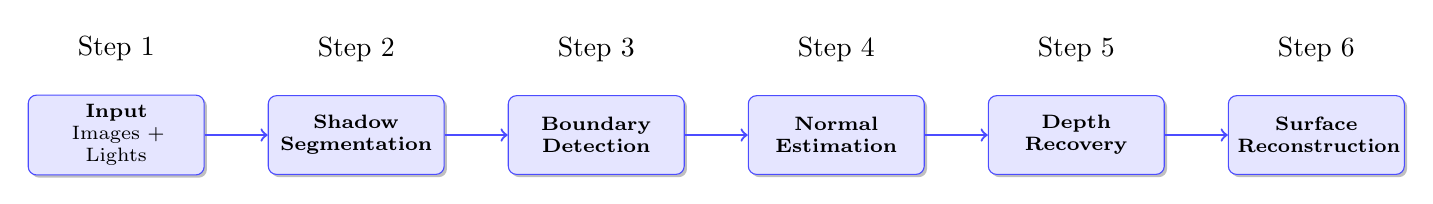
\begin{tikzpicture}[
    node distance=0.8cm,
    classicalbox/.style={rectangle, draw=blue!70, fill=blue!10, rounded corners=3pt, 
                        text width=2cm, text centered, minimum height=1cm, font=\scriptsize,
                        drop shadow={shadow xshift=1pt, shadow yshift=-1pt}},
    arrow/.style={->, thick, blue!70}
]

\node[classicalbox] (input) {\textbf{Input} \\ Images + Lights};
\node[classicalbox, right=of input] (shadow_seg) {\textbf{Shadow} \\ \textbf{Segmentation}};
\node[classicalbox, right=of shadow_seg] (boundary_det) {\textbf{Boundary} \\ \textbf{Detection}};
\node[classicalbox, right=of boundary_det] (normal_est) {\textbf{Normal} \\ \textbf{Estimation}};
\node[classicalbox, right=of normal_est] (depth_solve) {\textbf{Depth} \\ \textbf{Recovery}};
\node[classicalbox, right=of depth_solve] (surface_recon) {\textbf{Surface} \\ \textbf{Reconstruction}};

\draw[arrow] (input) -- (shadow_seg);
\draw[arrow] (shadow_seg) -- (boundary_det);
\draw[arrow] (boundary_det) -- (normal_est);
\draw[arrow] (normal_est) -- (depth_solve);
\draw[arrow] (depth_solve) -- (surface_recon);

% Timeline
\node[above=0.3cm of input] {Step 1};
\node[above=0.3cm of shadow_seg] {Step 2};
\node[above=0.3cm of boundary_det] {Step 3};
\node[above=0.3cm of normal_est] {Step 4};
\node[above=0.3cm of depth_solve] {Step 5};
\node[above=0.3cm of surface_recon] {Step 6};

\end{tikzpicture}
\caption{Classical method (Sequential processing pipeline)}
\label{fig:classical_method}
\end{figure}

\begin{figure}[htbp]
\centering
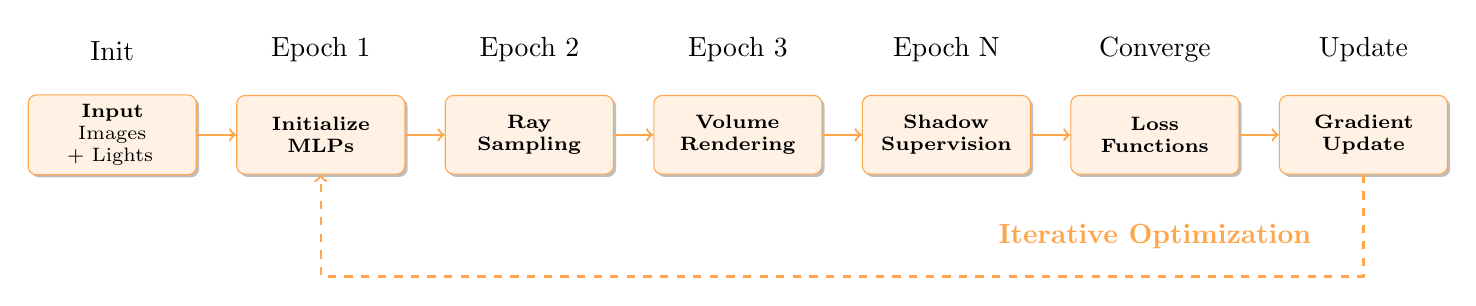
\begin{tikzpicture}[
    node distance=0.5cm,
    neuralbox/.style={rectangle, draw=orange!70, fill=orange!10, rounded corners=3pt,
                     text width=1.9cm, text centered, minimum height=1cm, font=\scriptsize,
                     drop shadow={shadow xshift=1pt, shadow yshift=-1pt}},
    arrow/.style={->, thick, orange!70},
]

\node[neuralbox] (input) {\textbf{Input} \\ Images + Lights};
\node[neuralbox, right=of input] (init_mlp) {\textbf{Initialize} \\ \textbf{MLPs}};
\node[neuralbox, right=of init_mlp] (ray_sample) {\textbf{Ray} \\ \textbf{Sampling}};
\node[neuralbox, right=of ray_sample] (volume_render) {\textbf{Volume} \\ \textbf{Rendering}};
\node[neuralbox, right=of volume_render] (shadow_super) {\textbf{Shadow} \\ \textbf{Supervision}};
\node[neuralbox, right=of shadow_super] (loss_compute) {\textbf{Loss} \\ \textbf{Functions}};
\node[neuralbox, right=of loss_compute] (gradient_update) {\textbf{Gradient} \\ \textbf{Update}};

\draw[arrow] (input) -- (init_mlp);
\draw[arrow] (init_mlp) -- (ray_sample);
\draw[arrow] (ray_sample) -- (volume_render);
\draw[arrow] (volume_render) -- (shadow_super);
\draw[arrow] (shadow_super) -- (loss_compute);
\draw[arrow] (loss_compute) -- (gradient_update);

\draw[arrow, dashed] (gradient_update) -- ++(0,-1.8) -| (init_mlp);
\node[below=of loss_compute, text=orange!70] {\textbf{Iterative Optimization}};

% Timeline
\node[above=0.3cm of input] {Init};
\node[above=0.3cm of init_mlp] {Epoch 1};
\node[above=0.3cm of ray_sample] {Epoch 2};
\node[above=0.3cm of volume_render] {Epoch 3};
\node[above=0.3cm of shadow_super] {Epoch N};
\node[above=0.3cm of loss_compute] {Converge};
\node[above=0.3cm of gradient_update] {Update};

\end{tikzpicture}
\caption{ShadowNeuS (End-to-end neural optimization pipeline)}
\label{fig:neural_method}
\end{figure}

\subsection{From Classical Shadow Analysis to Neural Methods} \label{sec:classical_to_neural}

Classical shadow-based 3D reconstruction (Figure~\ref{fig:classical_method}) uses a sequential pipeline: segmenting shadows, detecting boundaries, estimating normals, solving for depth, and reconstructing surfaces. This approach faces challenges like non-differentiable occlusion tests and circular dependencies between normals and depth, as detailed in Section~\ref{sec:shadow_limitations}.

ShadowNeuS (Figure~\ref{fig:neural_method}) overcomes these by representing the 3D scene as a neural Signed Distance Function (SDF) parameterized by a Multi-Layer Perceptron (MLP). It employs differentiable ray tracing and optimization to learn geometry from shadow or RGB images under multiple lighting conditions, resolving single-view ambiguities.

\begin{definition}[Neural Signed Distance Function] \label{def:neural_sdf}
A neural SDF \( f(\mathbf{x}; \theta): \mathbb{R}^3 \to \mathbb{R} \), parameterized by an MLP with weights \(\theta\), represents a 3D scene as follows:
\begin{itemize}
    \item \textbf{Surface}: \( f(\mathbf{x}) = 0 \) defines the surface \( \mathcal{S} \).
    \item \textbf{Outside}: \( f(\mathbf{x}) > 0 \), where \( f(\mathbf{x}) \) is the distance to the nearest surface point.
    \item \textbf{Inside}: \( f(\mathbf{x}) < 0 \), where \( |f(\mathbf{x})| \) is the distance to the surface.
    \item \textbf{Normal}: \( \nabla f(\mathbf{x}) \) is the surface normal at \( \mathbf{x} \in \mathcal{S} \), with \( \|\nabla f(\mathbf{x})\|_2 = 1 \).
\end{itemize}
\end{definition}

\begin{itemize}
    \item \textbf{SDF Use Cases in ShadowNeuS}:
        \begin{itemize}
            \item \textbf{If \( f(\mathbf{x}) = 0 \)}: The point \(\mathbf{x}\) lies on the surface. Used in camera ray marching to find surface points for rendering or shadow ray starting points.
                \begin{itemize}
                    \item \textit{Example}: A ray hits a surface point \(\hat{\mathbf{x}}\) where \( f(\hat{\mathbf{x}}) \approx 0 \), used to compute shadows or colors.
                \end{itemize}
            \item \textbf{If \( f(\mathbf{x}) > 0 \)}: The point is outside the object. The SDF value indicates how far \(\mathbf{x}\) is from the surface, guiding ray marching to approach the surface.
                \begin{itemize}
                    \item \textit{Example}: During ray marching, if \( f(\mathbf{x}) = 0.1 \), move 0.1 units toward the surface along the ray.
                \end{itemize}
            \item \textbf{If \( f(\mathbf{x}) < 0 \)}: The point is inside the object. The negative value helps identify occlusion in shadow rays.
                \begin{itemize}
                    \item \textit{Example}: A shadow ray passing through a point with \( f(\mathbf{x}) < 0 \) indicates occlusion, reducing radiance.
                \end{itemize}
        \end{itemize}
    \item \textbf{Gradient \( \nabla f(\mathbf{x}) \)}:
        \begin{itemize}
            \item \textbf{Definition}: \( \nabla f(\mathbf{x}) = \left( \frac{\partial f}{\partial x}, \frac{\partial f}{\partial y}, \frac{\partial f}{\partial z} \right) \) points toward the nearest surface and indicates the rate of SDF
            \item \textit{Example}: If a shadow ray hits a surface \(f(\hat{\mathbf{x})=0\), \( \nabla f(\hat{\mathbf{x}}) \) is the surface normal that determines if the point is lit or shadowed based on the tangency condition (Equation~\eqref{eq:tangency}).
        \end{itemize}
    \newpage
    \item \textbf{Norm-2 of Gradient \( \|\nabla f(\mathbf{x})\|_2 = 1 \)}:
        \begin{itemize}
            \item \textbf{True Distance Function}: An SDF is a \textit{true distance function} if \( f(\mathbf{x}) \) equals the Euclidean distance to the nearest surface, ensured by \( \|\nabla f(\mathbf{x})\|_2 = 1 \). This means moving a distance \( \delta \) in the gradient direction changes \( f(\mathbf{x}) \) by exactly \( \delta \).
            \item \textbf{Taylor Series Insight}: The first-degree Taylor approximation of \( f(\mathbf{x} + \delta \mathbf{u}) \) near \(\mathbf{x}\):
                \[
                f(\mathbf{x} + \delta \mathbf{u}) \approx f(\mathbf{x}) + \delta \nabla f(\mathbf{x}) \cdot \mathbf{u}
                \]
                If \( \mathbf{u} = \nabla f(\mathbf{x}) / \|\nabla f(\mathbf{x})\|_2 \) (unit direction) and \( \|\nabla f(\mathbf{x})\|_2 = 1 \), then:
                \[
                f(\mathbf{x} + \delta \nabla f(\mathbf{x})) \approx f(\mathbf{x}) + \delta
                \]
                This constant rate of change (factor of 1) ensures predictable updates in gradient descent and accurate ray marching steps.
            \item \textbf{Use Case}: The Eikonal constraint \( \|\nabla f\|_2 = 1 \) ensures:
                \begin{itemize}
                    \item \textit{Ray Marching}: Consistent step sizes to reach \( f(\mathbf{x}) = 0 \).
                    \item \textit{Gradient Descent}: Stable optimization by providing a constant scaling factor for MLP weight updates.
                    \item \textit{Normals}: Correctly scaled normals for shadow and RGB rendering.
                \end{itemize}
            \item \textit{Example}: If \( \|\nabla f\|_2 = 2 \), a step of 0.1 units in the gradient direction changes \( f(\mathbf{x}) \) by 0.2, causing ray marching to overshoot the surface and distorting shadows.
        \end{itemize}
\end{itemize}
    \item \textbf{Norm-2 of Gradient \( \|\nabla f(\mathbf{x})\|_2 = 1 \)}:
        \begin{itemize}
            \item \textbf{True Distance Function}: An SDF is a \textit{true distance function} if \( f(\mathbf{x}) \) equals the Euclidean distance to the nearest surface, ensured by \( \|\nabla f(\mathbf{x})\|_2 = 1 \). This means moving a distance \( \delta \) in the gradient direction changes \( f(\mathbf{x}) \) by exactly \( \delta \).
            \item \textbf{Taylor Series Insight}: The first-degree Taylor approximation of \( f(\mathbf{x} + \delta \mathbf{u}) \) near \(\mathbf{x}\):
                \[
                f(\mathbf{x} + \delta \mathbf{u}) \approx f(\mathbf{x}) + \delta \nabla f(\mathbf{x}) \cdot \mathbf{u}
                \]
                If \( \mathbf{u} = \nabla f(\mathbf{x}) / \|\nabla f(\mathbf{x})\|_2 \) (unit direction) and \( \|\nabla f(\mathbf{x})\|_2 = 1 \), then:
                \[
                f(\mathbf{x} + \delta \nabla f(\mathbf{x})) \approx f(\mathbf{x}) + \delta
                \]
                This constant rate of change (factor of 1) ensures predictable updates in gradient descent and accurate ray marching steps.
            \item \textbf{Use Case}: The Eikonal constraint \( \|\nabla f\|_2 = 1 \) ensures:
                \begin{itemize}
                    \item \textit{Ray Marching}: Consistent step sizes to reach \( f(\mathbf{x}) = 0 \).
                    \item \textit{Gradient Descent}: Stable optimization by providing a constant scaling factor for MLP weight updates.
                    \item \textit{Normals}: Correctly scaled normals for shadow and RGB rendering.
                \end{itemize}
            \item \textit{Example}: If \( \|\nabla f\|_2 = 2 \), a step of 0.1 units in the gradient direction changes \( f(\mathbf{x}) \) by 0.2, causing ray marching to overshoot the surface and distorting shadows.
        \end{itemize}
\end{itemize}
        \alpha_i = \max \left( 1 - \frac{\Phi_s(f(\mathbf{p}(t_{i+1}); \theta))}{\Phi_s(f(\mathbf{p}(t_i); \theta))}, 0 \right), \quad \Phi_s(z) = \frac{1}{1 + e^{-sz}}
        \]
        Compute radiance:
        \[
        \hat{C}_{\text{in}}(\hat{\mathbf{x}}, \mathbf{L}_i) = L \prod_{i=1}^N (1 - \alpha_i)
        \]
        where \(L\) is the light intensity (assumed constant).
    \item \textbf{RGB Rendering (Optional)}: For RGB images, compute color at \(\hat{\mathbf{x}}\):
        \[
        \hat{C} = (\rho_d + \rho_s) \hat{C}_{\text{in}} (\mathbf{L}_i - \hat{\mathbf{x}}) \cdot \nabla f(\hat{\mathbf{x}})
        \]
        where \(\rho_d\) and \(\rho_s\) are diffuse and specular reflectance coefficients.
    \item \textbf{Loss Computation}: Compute the shadow or RGB loss to enforce consistency with input images:
        \[
        \mathcal{L}_{\text{shadow}} = \|\hat{C}_{\text{in}} - I_s\|_1, \quad \mathcal{L}_{\text{rgb}} = \|\hat{C} - I_r\|_1
        \]
        where \(I_s\) is the binary shadow image and \(I_r\) is the RGB image. Add the Eikonal loss to ensure a valid SDF:
        \[
        \mathcal{L}_{\text{eik}} = \frac{1}{M} \sum_{i=1}^M \left( \|\nabla f(\mathbf{p}_i; \theta)\|_2 - 1 \right)^2
        \]
        Combine losses:
        \[
        \mathcal{L} = \mathcal{L}_{\text{shadow/rgb}} + 0.01 \cdot \mathcal{L}_{\text{eik}}
        \]
    \item \textbf{Gradient Update}: Use the Adam optimizer to update MLP weights \(\theta\) by minimizing \(\mathcal{L}\) over 150,000 iterations, with a coarse-to-fine strategy (100x100 to 800x800 image resolution).
\end{enumerate}

\begin{remark}[Differentiable Pipeline]
The neural SDF and ray tracing are fully differentiable, allowing gradients to flow from the loss to \(\theta\), enabling end-to-end optimization of geometry and appearance.
\end{remark}

\subsubsection{Addressing Classical Limitations} \label{sec:address_limitations}

ShadowNeuS overcomes the challenges listed in Section~\ref{sec:shadow_limitations} as follows:

\begin{enumerate}[label=\arabic*.]
    \item \textbf{Circular Dependency}: The neural SDF provides both geometry (\(f(\mathbf{x})\)) and normals (\(\nabla f(\mathbf{x})\)) simultaneously, resolving the need for separate normal estimation.
    \item \textbf{Singular Cases}: The Eikonal loss ensures \(\|\nabla f\|_2 = 1\), stabilizing normals near grazing angles.
    \item \textbf{Non-Unique Solutions}: Multiple lighting conditions (\(\{\mathbf{L}_i\}\)) provide diverse shadow cues, reducing ambiguity in depth recovery.
    \item \textbf{Non-Differentiable Occlusion}: The continuous SDF and sigmoid-based opacity \(\Phi_s\) enable differentiable shadow ray tracing, replacing discrete intersection tests.
    \item \textbf{Nonlinear Systems}: The shadow loss \(\mathcal{L}_{\text{shadow}}\) implicitly enforces tangency constraints (Equation~\eqref{eq:tangency}) through optimization, avoiding explicit solvers.
    \item \textbf{Ray Tracing Complexity}: GPU-based parallel processing and batched ray sampling reduce computational cost compared to classical \(O(n^2)\) methods.
    \item \textbf{Light Localization}: Known light positions \(\{\mathbf{L}_i\}\) eliminate estimation errors, though robust loss functions can mitigate minor inaccuracies.
    \item \textbf{Shadow Detection}: The L1 loss is robust to soft shadows and noise, as it compares entire shadow maps rather than relying on precise boundary detection.
    \item \textbf{Multi-Object Complexity}: The neural SDF implicitly represents all surfaces, handling self-shadowing and multiple occluders by evaluating \(f(\mathbf{x})\) along rays.
\end{enumerate}

\begin{remark}[Shadow Cues in ShadowNeuS]
Shadows provide geometric cues (surface orientation, tangency, depth ordering, occlusion) that constrain the SDF to match observed shadow boundaries and cast shadows across multiple lighting conditions, enabling reconstruction of complex geometries.
\end{remark}

\subsubsection{Shadow Consistency Loss} \label{sec:shadowneus_loss}

\begin{definition}[Shadow Consistency Loss] \label{def:shadowneus_loss}
The shadow consistency loss in ShadowNeuS is:
\begin{equation}
\boxed{\mathcal{L}_{\text{shadow}} = \|\hat{C}_{\text{in}} - I_s\|_1} \label{eq:shadowneus_loss}
\end{equation}
where \(\hat{C}_{\text{in}}\) is the predicted radiance from shadow ray tracing, and \(I_s\) is the observed binary shadow image.
\end{definition}

\begin{remark}[Comparison to Classical Loss]
Unlike the classical shadow consistency loss (Equation~\ref{def:shadow_loss}), which uses weighted terms for lit, shadow, and boundary mismatches, ShadowNeuS simplifies to a single L1 loss over all pixels. This leverages the neural SDF’s ability to implicitly handle boundaries and regions through differentiable rendering.
\end{remark}

\begin{proposition}[Geometric Constraints via Shadows]
The shadow loss enforces:
\begin{itemize}
    \item \textbf{Surface Orientation}: Points in \(\Omega_{\text{shadow}}^{\text{obs}}\) correspond to \(\mathcal{S}_{\text{shadow}}\) or \(\mathcal{C}_{\text{total}}\), constraining \(\nabla f(\mathbf{x})\).
    \item \textbf{Tangency}: Pixels in \(\partial\Omega_{\text{shadow}}^{\text{obs}}\) satisfy Equation~\eqref{eq:tangency} implicitly through optimization.
    \item \textbf{Depth Ordering}: Cast shadows in \(\mathcal{C}_{\text{total}}\) ensure correct relative positioning of surfaces.
\end{itemize}
\end{proposition}

\begin{theorem}[Depth Recovery in ShadowNeuS]
For a pixel \(\vect{p} \in \partial\Omega_{\text{shadow}}^{\text{obs}}\), the depth \(\lambda\) is constrained by:
\begin{equation}
\boxed{(\mathbf{C} + \lambda \mathbf{d} - \mathbf{L}_i) \cdot \nabla f(\mathbf{C} + \lambda \mathbf{d}) = 0} \label{eq:shadowneus_depth}
\end{equation}
ShadowNeuS solves this implicitly by optimizing the SDF to match shadow images across multiple lights \(\{\mathbf{L}_i\}\).
\end{theorem}

\begin{proof}
For \(\vect{p} \in \partial\Omega_{\text{shadow}}^{\text{obs}}\), the 3D point \(\mathbf{P} = \mathbf{C} + \lambda \mathbf{d}\) lies on the shadow boundary \(\mathcal{B}\). The tangency condition (Equation~\eqref{eq:tangency}) applies, with \(\vect{n}(\mathbf{P}) = \nabla f(\mathbf{P})\), yielding Equation~\eqref{eq:shadowneus_depth}.
\end{proof}

\begin{remark}[Neural Optimization Advantage]
By optimizing \(\mathcal{L}_{\text{shadow}} + 0.01 \cdot \mathcal{L}_{\text{eik}}\) over multiple lighting conditions, ShadowNeuS resolves depth ambiguities without explicit normal estimation or iterative solvers, leveraging the MLP’s expressive power and gradient-based optimization.
\end{remark}

% \section{1D Shadow-Based Reconstruction Experiment} \label{sec:1d_experiment}

% \subsection{Problem Formulation: 2D Reconstruction from 1D Observations} \label{sec:1d_problem}

% \subsubsection*{Dimensional Reduction of ShadowNeuS} \label{sec:dimensional_reduction}

% % Content: Reducing 3D→2D problem to 2D→1D, mathematical simplification

% \subsubsection*{1D Shadow Projection Model} \label{sec:1d_projection}

% % Content: 1D camera model, light source, shadow formation in 2D→1D setting

% \subsubsection*{Mathematical Framework} \label{sec:1d_framework}

% % Content: 1D SDF, ray equations, shadow constraints in reduced dimension

% \subsection{Experimental Setup} \label{sec:experimental_setup}

% \subsubsection*{Synthetic 2D Scene Generation} \label{sec:2d_scene_gen}

% % Content: Creating test scenes, ground truth 2D shapes, lighting setup

% \subsubsection*{1D Shadow Profile Creation} \label{sec:1d_profile}

% % Content: Projecting 2D scenes to 1D observations, shadow profile extraction

% \subsubsection*{Network Architecture Design} \label{sec:1d_network}

% % Content: Simplified neural network for 1D→2D reconstruction, architectural choices

% \subsection{Implementation and Results} \label{sec:implementation_results}

% \subsubsection*{Training Protocol} \label{sec:training_protocol}

% % Content: Training procedure, hyperparameters, convergence criteria

% \subsubsection*{Reconstruction Quality Metrics} \label{sec:quality_metrics}

% % Content: Evaluation metrics, comparison with ground truth, quantitative results

% \subsubsection*{Comparison with Classical Methods} \label{sec:classical_comparison}

% % Content: Baseline comparisons, advantages of neural approach

% \subsection{Analysis and Insights} \label{sec:analysis_insights}

% \subsubsection*{Convergence Behavior} \label{sec:convergence_analysis}

% % Content: Training dynamics, loss evolution, stability analysis

% \subsubsection*{Shadow Constraint Effectiveness} \label{sec:shadow_effectiveness}

% % Content: Ablation studies, impact of shadow supervision

% \subsubsection*{Limitations and Future Directions} \label{sec:limitations_future}

% % Content: Current limitations, potential improvements, scaling to higher dimensions





\newpage

\section*{References}
\begin{tabular}{@{}p{0.1\textwidth} p{0.9\textwidth}}
\hypertarget{[LWX23]}{[LWX23]} & Jingwang Ling, Zhibo Wang, Feng Xu. \textit{ShadowNeuS: Neural SDF Reconstruction by Shadow Ray Supervision}. arXiv: \href{https://arxiv.org/abs/2211.14086}{2211.14086}, 2023.
\end{tabular}

\end{document}